\chapter{Messmethodik}
\section{Gasbox}

\begin{figure}[h]
	\centering
	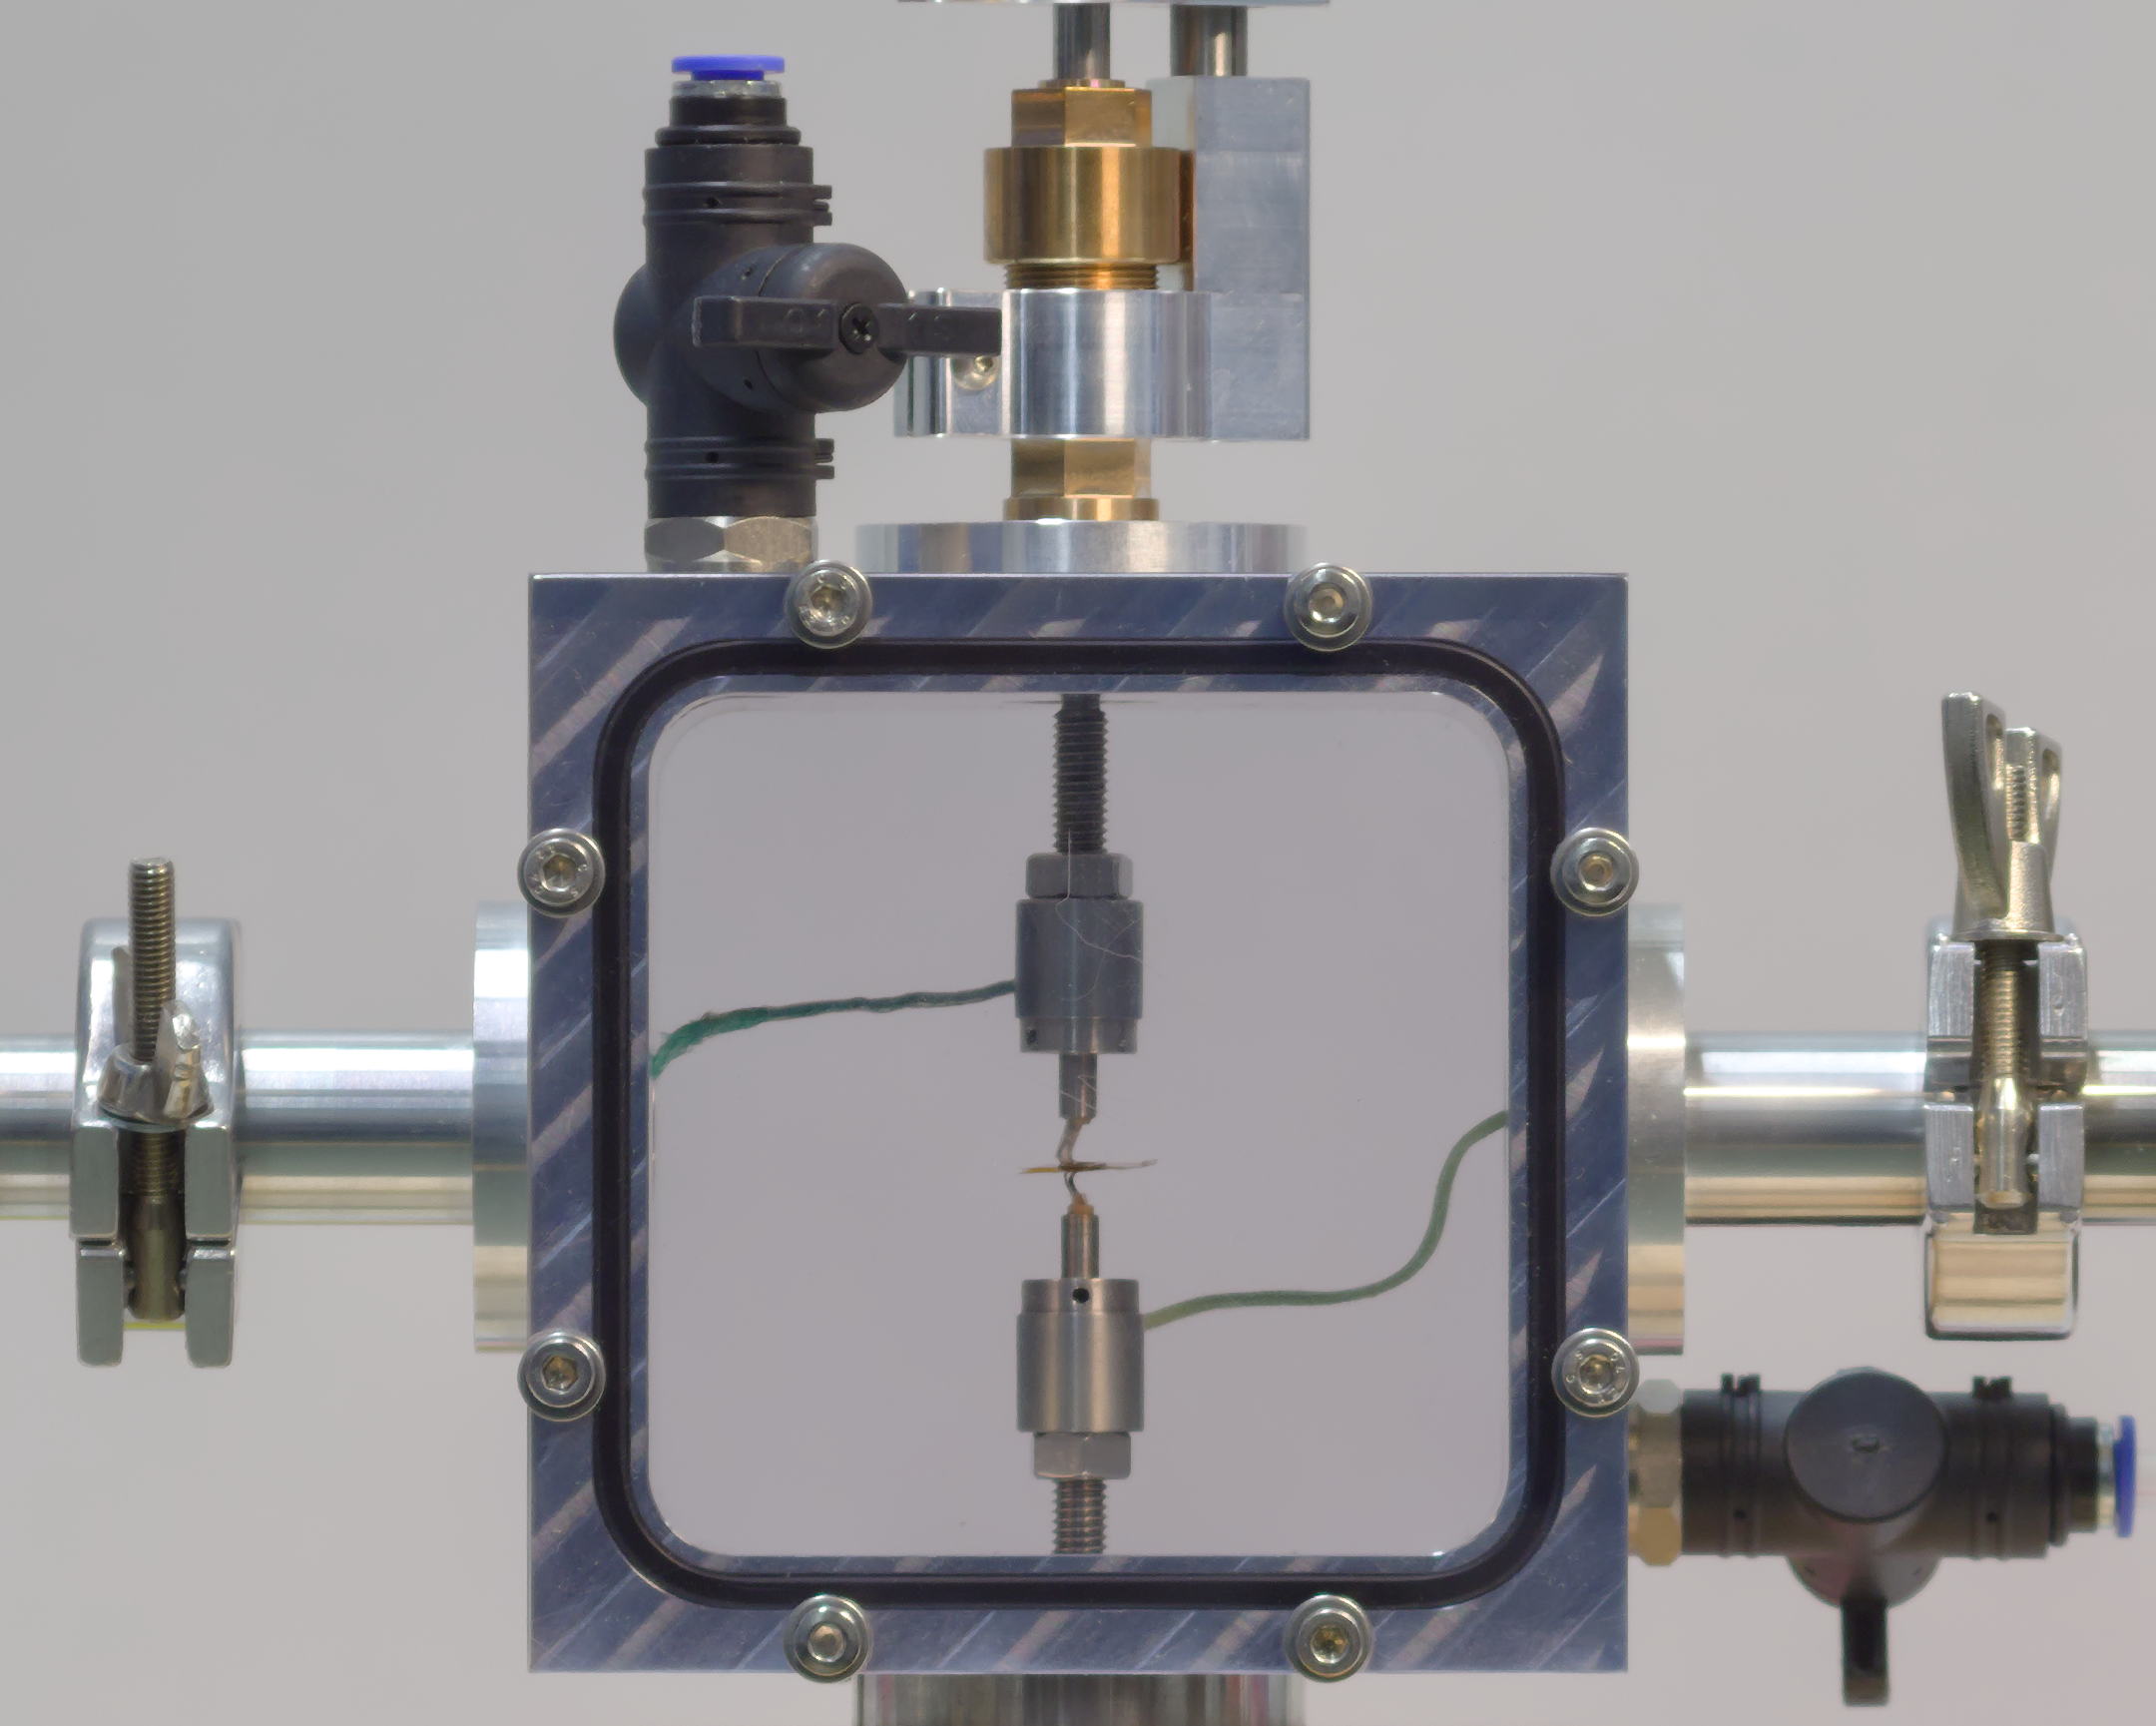
\includegraphics[width=0.8\linewidth]{bilder/gasbox_kleiner.png}
	\caption{Die Gasbox, in der das Plasma gezündet wird.}
	\label{fig:gasbox}
\end{figure}


Das Kernstück des Aufbaus ist die in Abb. \ref{fig:gasbox} abgebildete Gasbox, in der das Plasma gezündet wird. Die Box besteht aus Stahl mit zwei Fenstern zur Beobachtung und als Öffnung zum Einbau der PTPs. In dieser Box befinden sich zwei Thermosonden, die auch als Elektroden zum Zünden des Mikroplasmas dienen. Die untere Sonde ist auf ein festes Gewinde geschraubt, die obere Sonde ist senkrecht über eine Durchführung nach außen verschiebbar. Mit einer Mikrometerschraube ist die Höhe der Sonde fein einstellbar. Da die Position der Sondenplättchen auf den biegsamen Kabeln nicht vollständig fest ist, dient die Mikrometerschraube zwar zur feinen Einstellung, eignet sich aber nicht, um die Position mehrfach und reproduzierbar gleich einzustellen. Zur Einhaltung des Elektrodenabstandes wird daher ein dielektrischer Abstandshalter aus Kapton mit einem Loch in der Mitte als Zündraum verwendet. Die Kabel der Thermosonden werden durch Flansche zu den Ausleseplatinen geführt, die sich in T-Stücken auch in der Gasatmosphäre befinden. Dies vermeidet, die gewebeummantelten Kabel der PTPs nach außen führen zu müssen, was eine potenzielle Leckstelle wäre. Zudem gibt es noch zwei Gasanschlüsse als Ein- und Auslässe, entweder zum Durchspülen oder zum Abpumpen mit einer Vakuumpumpe. Dabei wird für Gase wie Helium, die leichter sind als Luft, das obere Ventil als Einlass genutzt, um die Luft in der Kammer nach unten durch das zweite Ventil zu verdrängen. Für dichtere Gase würden die Eingänge vertauscht. Über ein Manometer am Auslass lässt sich der Druck im Inneren der Kammer messen. Dieser Aufbau ist eine speziell auf PTP Messungen ausgelegte Weiterentwicklung der Gasbox aus \cite{hansenConventionalNonconventionalDiagnostics2022}, da mit geringerem Gasvolumen und ohne konstantes Spülen gearbeitet werden kann.


\section{Elektrischer Schaltplan}

\begin{figure}[h]
	\centering
	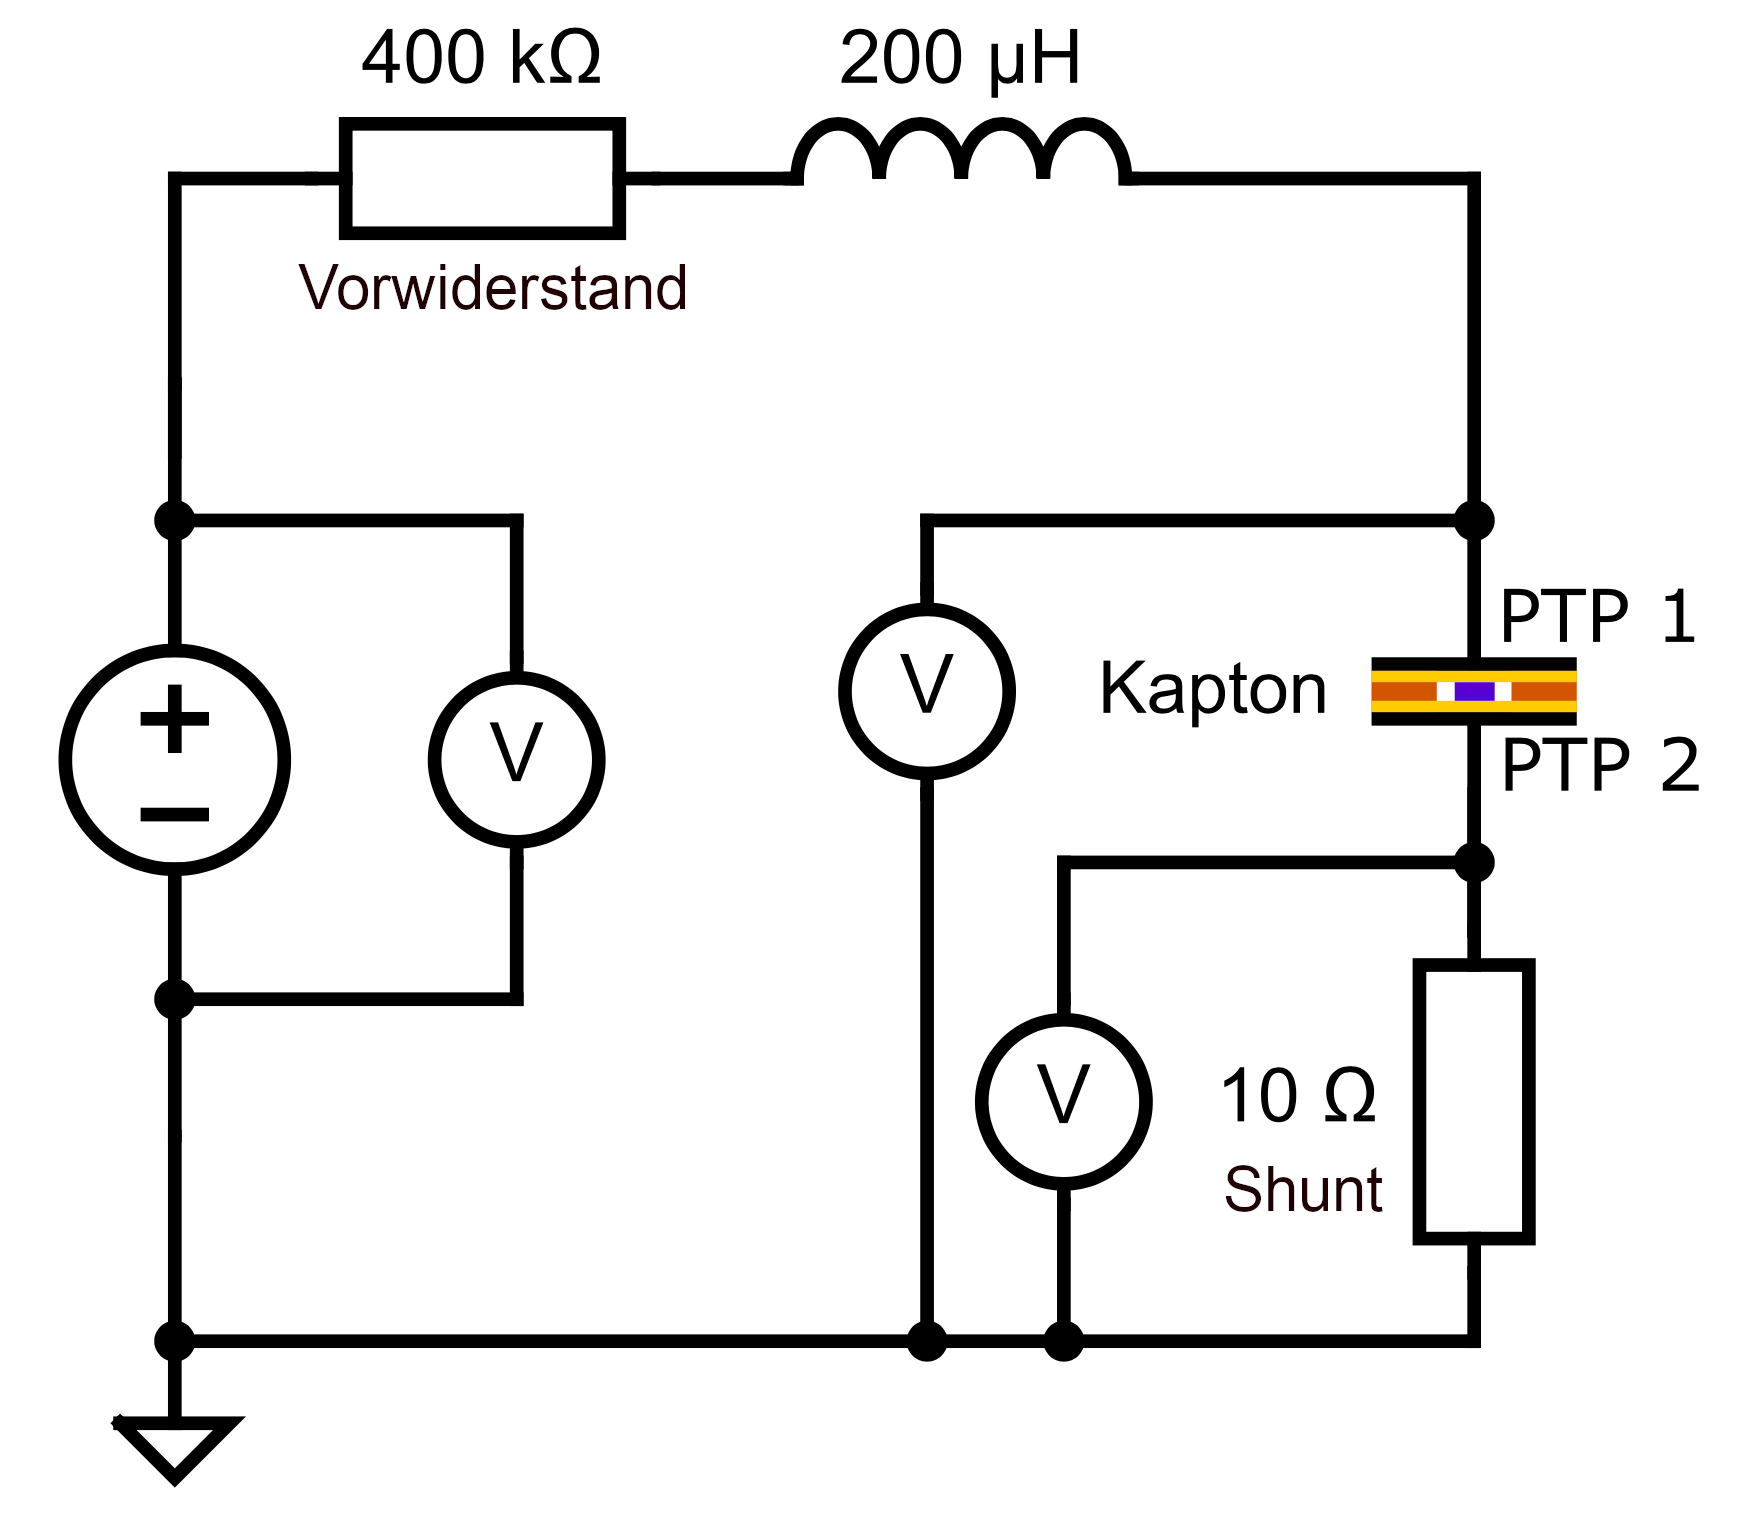
\includegraphics[width=0.5\linewidth]{bilder/schaltbild_beschriftet.png}
	\caption{Schaltbild des elektrischen Schaltkreises der Mikroplasmakammer. Als Elektroden dienen zwei PTPs. Hochspannungsmessköpfe messen die Spannungen am Netzteil, dem Mikroplasma und über dem Shunt-Widerstand. Bild aus \cite{hansenConventionalNonconventionalDiagnostics2022}.}
	\label{fig:schaltbild}
\end{figure}


Aus der Gasbox werden je PTP zweierlei Kabel herausgeführt. Zum einen werden über eine RS232-Verbindung die Daten der PTP-Platinen ausgelesen. Diese werden über einen galvanisch getrennten USB auf Seriell-Wandler (Delock 62502) an die Auswertungsrechner angeschlossen, was die Messung deutlich robuster gegenüber Stromstößen durch Arcing macht. Zudem wird über eine SHV-Stecker-Durchführung die elektrische Verbindung zum Plasma hergestellt. Der Schaltkreis für den Betrieb des Plasmas wird in Abb. \ref{fig:schaltbild} gezeigt. Von der Spannungsquelle (Heinzinger PNC 3500-300 ump) kommend, fließt der Strom zunächst durch eine Induktivität von \qty{200}{\micro\henry} und einen Vorwiderstand von \qty{400}{\kilo\ohm}. Danach wird er durch die Durchführung in die Gasbox geführt, wo das Plasma als Verbindung dient. Durch die zweite Durchführung wird der Strom nach außen und anschließend durch einen Shunt in die Erde geführt. Die elektronischen Daten werden mit drei Oszilloskoptastköpfen aufgenommen. Ein 1:1000 Tastkopf (Tektronix P6015A) misst zwischen Hochspannungseingang und Erde die gesamte von der Spannungsquelle ausgegebene Spannung. Ein 1:100 Tastkopf (Tektronix P5100A) wird nach dem Vorwiderstand angelegt und misst die über dem Plasma abfallende Spannung. Ein 1:1 Tastkopf (Tektronix P2200) misst schließlich über den Shunt den durch das Plasma fließenden Strom. Die von den Tastköpfen gemessenen Daten werden über ein Oszilloskop\footnote{PicoScope 5442B} ausgelesen und gespeichert.

\section{Elektroden und Aufbau des Mikroplasmas}

\begin{figure}[h]
	\centering
	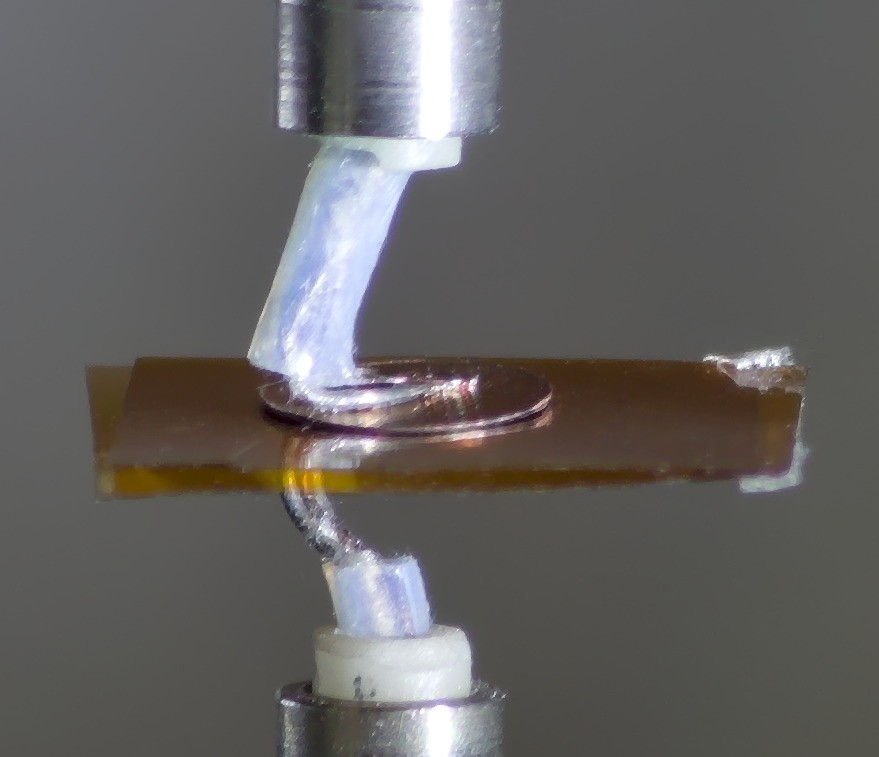
\includegraphics[width=0.7\linewidth]{bilder/plaettchenbesser.jpg}
	\caption{Nahaufnahme der eingebauten Elektroden samt Kaptonfolie.}
	\label{fig:plaettchen}
\end{figure}

Zwischen den beiden PTP-Plättchen als Elektroden wird das Mikroplasma gezündet. Um den Abstand von \qty{100}{\um} sicherzustellen, wird zwischen den Sonden eine zweilagige Kapton-Folie eingelegt, in der sich ein Loch von 1mm Durchmesser befindet. Auf diese Folie werden mit leichtem Druck die Sonden angedrückt, was sowohl die Folie glättet, als auch die Sondenplättchen parallel zueinander ausrichtet, da diese an den etwas biegsamen Verbindungsdrähten befestigt sind. Kapton wird als dielektrischer Abstandshalter benutzt, da es hitzebeständig und durchschlagfest ist und bei Unterdruck nicht ausgast. Abb. \ref{fig:plaettchen} zeigt eine Nahaufnahme dieser Elektroden.

\section{Ablauf der Energiestrommessungen}\label{sec:ablauf_energie}

Im Laufe der Energiestrommessungen wird für jedes Elektrodenmaterial die gleiche Messreihe durchgeführt. Dabei wird die Leistung des Plasmas auf die Elektroden für verschiedene Spannungen am Netzteil und damit für verschiedene Gesamtleistungen vermessen. Da mindestens \qty{500}{V} zur Zündung der Entladung benötigt werden (siehe \ref{sec:zuendspannung}), ist dies eine untere Grenze für den messbaren Bereich. Um ausreichend über der Zündspannung zu arbeiten und keine zu hohen Leistungen zu nutzen, wurden Werte von \qtyrange{700}{1000}{V} in \qty{50}{V} Schritten in sowohl positiver als auch negativer Polarität genutzt.

Im Laufe der Messreihe wird von \qty{700}{V} aufwärts gemessen, wobei die \qty{700}{V}-Messung zur Prüfung der Vergleichbarkeit am Ende der Reihe wiederholt wird. 
Die Messung bei einem Spannungswert besteht dabei aus sechs der in \ref{messprinzip} beschriebenen Temperaturpeaks. Bei jedem dieser Peaks ist das Mikroplasma dabei jeweils für \qty{10}{s} an- und dann für \qty{30}{s} ausgeschaltet. In \qty{10}{s} kann eine ausreichend lange Temperaturzeitreihe aufgenommen werden, um die dT-Auswertung zu benutzen und der Einfluss von zeitabhängigen Abweichungen beim Umschalten des Plasmas wird begrenzt. Gleichzeitig bleiben die äußeren Bedingungen, besonders die Außentemperatur, auf dieser Zeitskala unverändert, was eine wichtige Annahme der Auswertungsmethode rechtfertigt. In den \qty{30}{s}, für die das Plasma ausgeschaltet bleibt, ist genug Zeit, dass die Temperatur der Sonden auf weniger als \qty{0,5}{\celsius} über der Ausgangstemperatur vor der Messung absinkt. Dies gewährleistet eine Vergleichbarkeit der Messpeaks untereinander, da sich die Grundtemperatur im Laufe der Messung nicht relevant erhöht.

Die Wirkungsgrade und ESEEC werden aus der Messreihe für jede Spannung einzeln berechnet und gemittelt. Damit baut ein gemessener Sekundärelektronenkoeffizient auf den Messdaten von 42 Messpeaks auf\footnote{Bzw. 84, wenn auch über beide Polungen gemittelt wird.}, was den statistischen Fehler gering hält. Bei Kupfer wurde zusätzlich eine zweite dieser Messreihen bei vertauschten Sonden durchgeführt, um zu überprüfen, ob eine im Messprozess ggf. bewirkte Änderung der Oberflächenstruktur einen Einfluss auf die ESEEC hat. Da sich kein signifikanter Unterschied der ESEEC ergab, wurde der schlussendliche Koeffizient aus dem Mittelwert beider Messungen gebildet, womit pro Spannung und Polung effektiv 12 statt 6 Messpeaks genutzt wurden.

\section{Aufbau der optischen Emissionsspektroskopie (OES)}

Um die Gasreinheit innerhalb des Plasmas zu überprüfen, wurden optische Emissionsspektren der Entladung aufgenommen. Dafür wurde eine Glasfaser mit einer Fokussierungslinse auf die Entladung ausgerichtet, die die Strahlung dann in ein Spektroskop (OceanOptics HR2000+CG-UV-NIR) leitet. Pro Messung wurde dabei je ein Hell- und ein Dunkelspektrum aufgenommen, um systematische Fehler herauszurechnen. Da aus vorherigen Arbeiten bekannt ist, dass die Emissionsspektren während des Betriebs des Mikroplasmas konstant bleiben \cite{hansenConventionalNonconventionalDiagnostics2022}, wurde hier nur alle zehn Minuten ein Spektrum aufgenommen, um die Gasreinheit zu kontrollieren.